\documentclass[12pt, letterpaper]{article}
\usepackage[utf8]{inputenc}
\usepackage[italian]{babel}
\usepackage[T1]{fontenc}
\usepackage{graphicx}
\graphicspath{}

\title{Progetto per il corso di Progetto Automatico di Sistemi Digitali}
\author{Filippo Landi}

\begin{document}
\maketitle

\begin{abstract}
Il mio progetto per il corso di Progetto Automatico di Sistemi Digitali (PASD in breve) consiste nello studio statistico del comportamento di un circuito "multiply and accumulate" (o "mac" in breve) in presenza di alcuni difetti di produzione.
\end{abstract}

\section{Introduzione al progetto}

Il progetto riguarda il collaudo dei sistemi digitali, argomento del corso di PASD.

Al fine di simulare i guasti del circuito userò "HOPE" un simulatore di guasto per circuiti digitali sequenziali sviluppato dall'università VirginiaTech, anche questo proposto durante il corso.  

HOPE legge i circuiti attraverso delle descrizioni della rete (netlist) in formato .bench, quindi il primo punto del progetto sarà studiare la struttura del circuito per implementarlo in questo formato.

Ho deciso di usare Python per aiutarmi con i diversi passaggi del progetto.

Partiamo quindi dalla descrizione del circuito da studiare, passeremo poi alla sua implementazione e in fine ad alcuni studi statistici.

\section{Circuito multiply and accumulate}

Mi è stato richiesto di realizzare un circuito multiply and accumulate (mac) a 8 bit, esso è composto da un moltiplicatore con un sommatore in cascata e un registro per retroazionare le uscite in modo da accumulare i risultati.

Riporto un documento inviatomi dal professore che illustra gli schemi di un circuito di questo tipo a 4 bit.

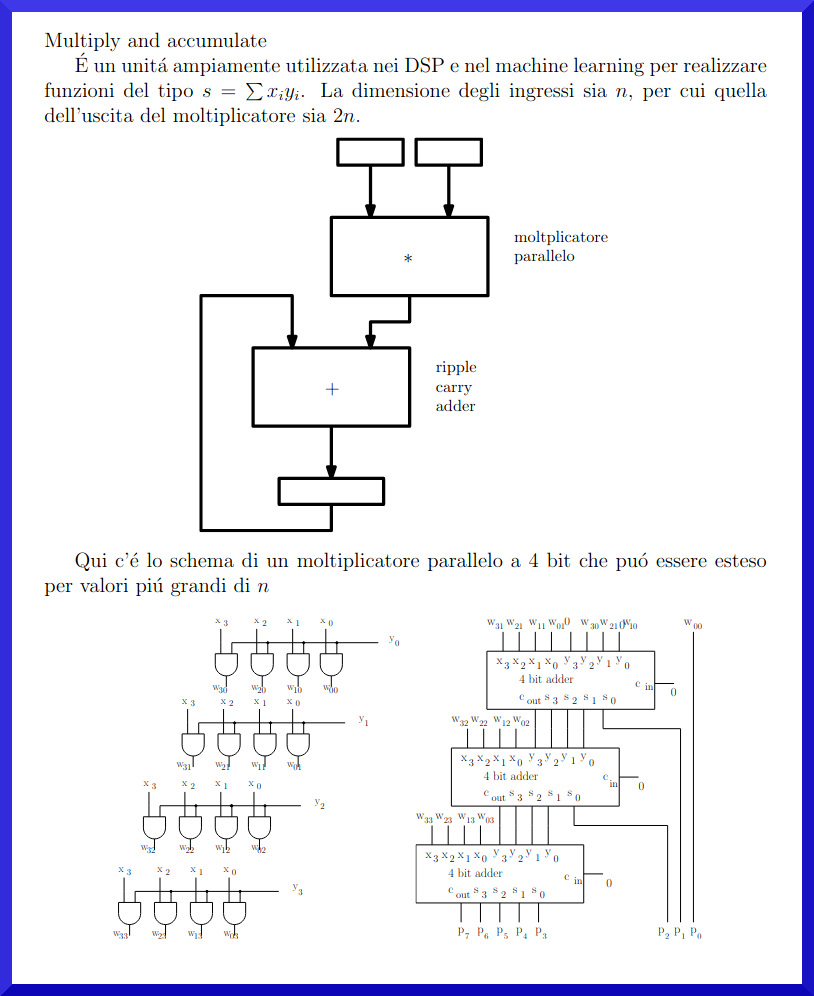
\includegraphics[width=13cm]{mac.png}

\newpage
\subsection{Moltiplicatore}
La struttura del moltiplicatore è ben illustrata nella documentazione:

\begin{itemize}
  \item Ogni segnale X è messo in AND con ogni Y, generando i segnali W.
  \item I segnali W vengono usati da degli adder strutturati su più livelli: si può notare che il numero di livelli è n-1 in quanto al primo livello vengono usati WX1 e WX0, poi i rimanenti WXY nei livelli successivi.
\end{itemize}

\subsection{Sommatore}
È un ripple carry adder con dimensione degli ingressi 2n: un ingresso è dato dall'uscita del moltiplicatore mentre l'altra è data dalle uscite stesse del sommatore retroazionate attraverso dei flip flop tipo D (circuito già integrato in HOPE).

\subsubsection{Ripple Carry Adder}

Usiamo dei ripple carry adder sia per la cascata di adder del moltiplicatore oltre che per il ripple carry adder successivo con dimensione degli ingressi 2n.

I ripple carry adder nella precedente documentazione erano illustrati a livello register transfer level (RTL) per ovvie ragioni di chiarezza, però per l'implementazione del circuito ci serve vedere come sono fatti a livello di porte logiche.  

I ripple carry adder sono circuiti formati da una serie di adder in cascata:
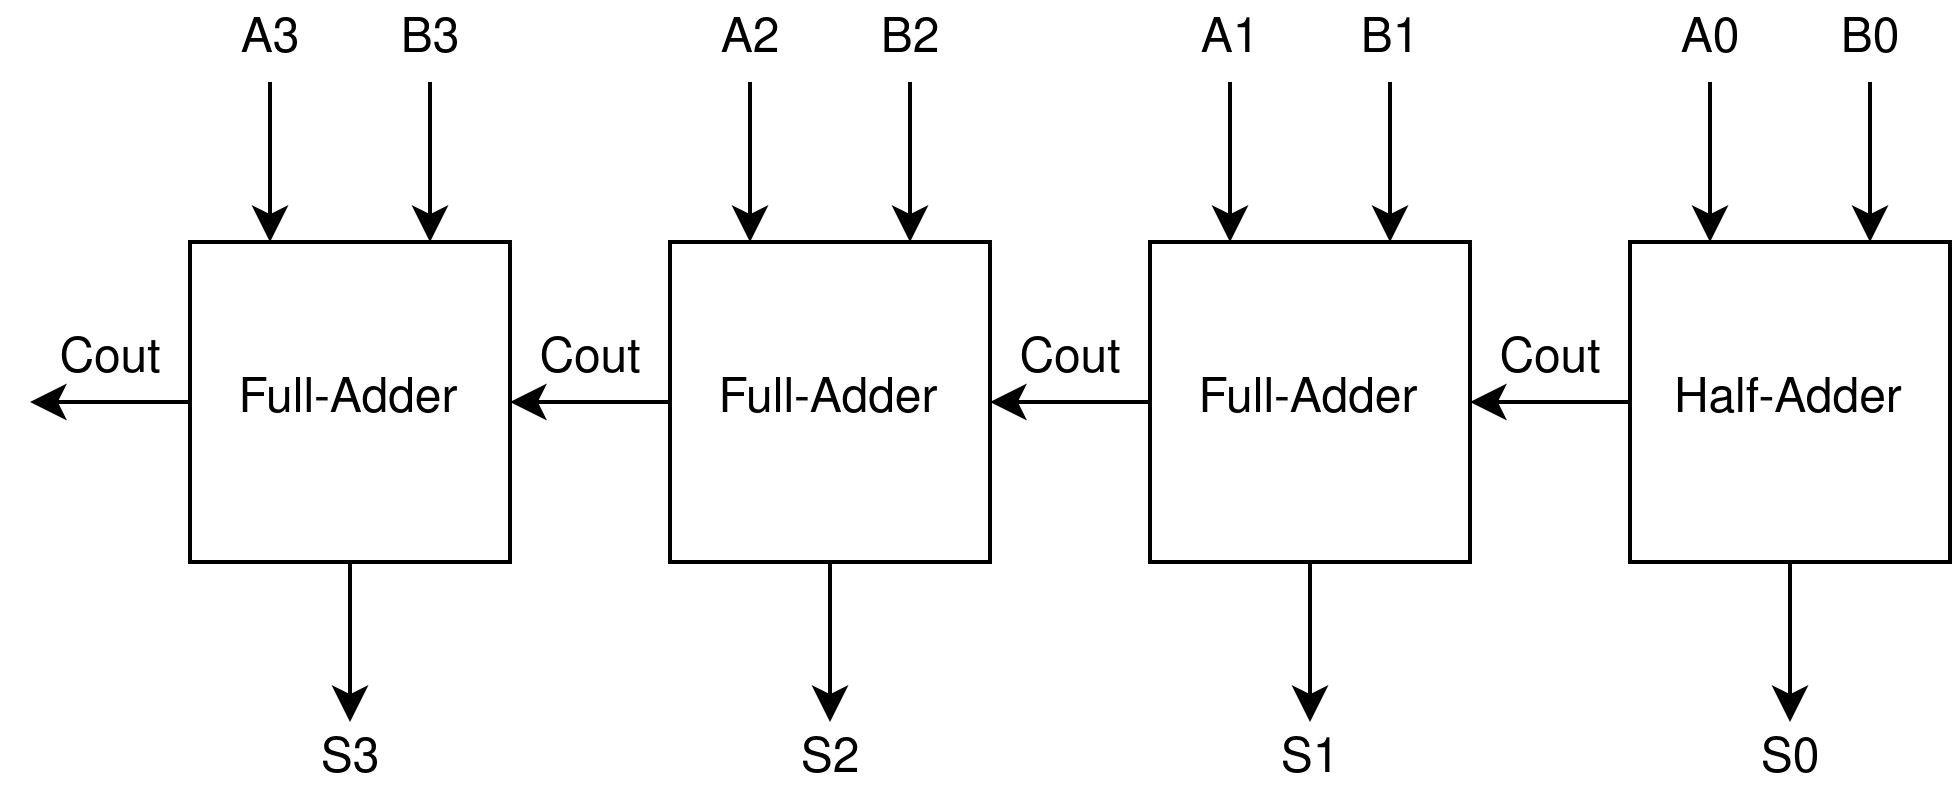
\includegraphics[width=\textwidth]{ripple_carry_adder}

Questo è lo schema che uso del half-adder:
\begin{center}

\includegraphics{half_adder}
\end{center}

Questo è lo schema che uso del full-adder:
\begin{center}
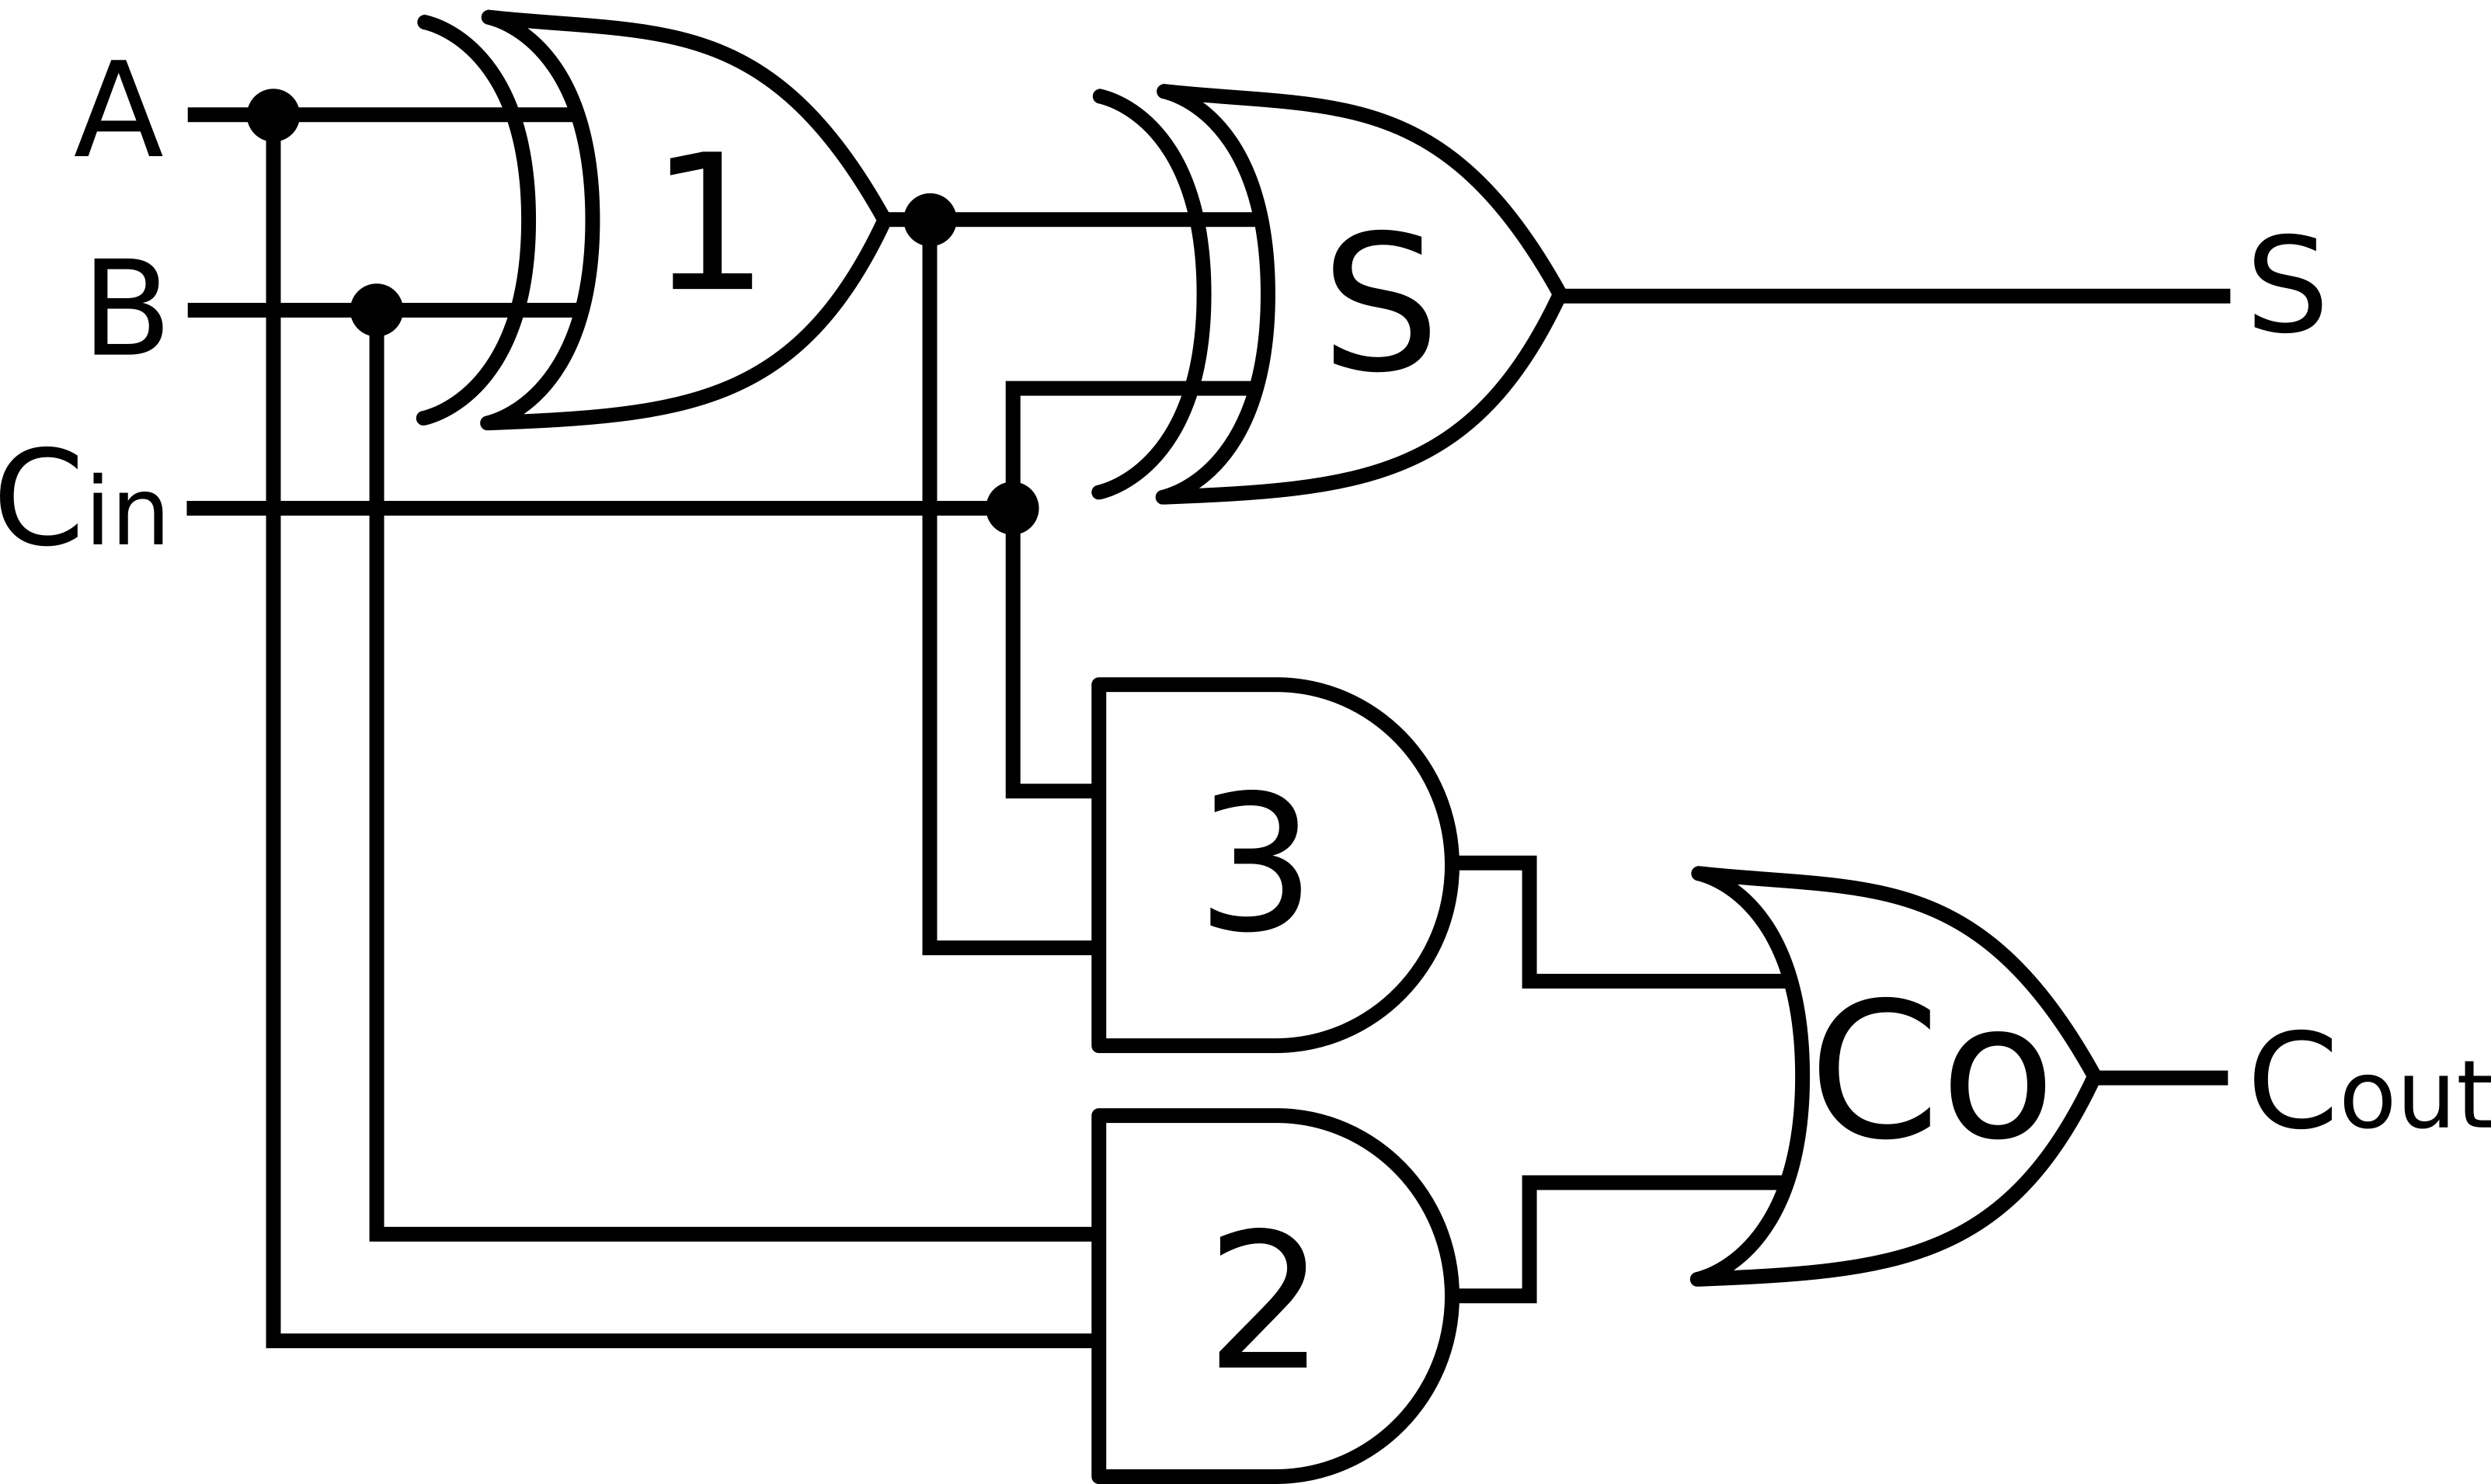
\includegraphics[width=8cm]{full_adder}
\end{center}

Opportunamente collegando le varie porte logiche quindi si ottiene un ripple carry adder.  

\section{Realizzazione del circuito in .bench}

La stesura manuale del file .bench del circuito ad 8 bit non mi sembrava un approccio furbo vista l'architettura piuttosto complessa da rappresentare. Probabilmente proseguire con tale metologia avrebbe portato a vari errori: sia banalmente di battitura, sia dovuti alla complessità e quindi errori nel collegamento dei vari segnali. Per questo ho pensato ad una metodologia stile "divide et impera".

In partenza ho scritto alcuni circuiti di prova per esplorare i vari adder e la prima parte del moltiplicatore.
Li trovate nella cartella "circuti\_prova", non sono fondamentali per il progetto però possono aiutare alla comprensione della metodologia usata.

Appurata la struttura dei circuiti base ho creato un singolo file che li mettesse insieme in maniera opportuna (vari cicli for più certe condizioni).
Questo approccio ha portato allo script "mac\_generator.py" che permette di generare il circuito con una dimensione arbitraria degli ingressi da passare come argomento: per generare un mac 4 bit si può scrivere da terminale questo comando Python: "python3 mac\_generator.py 4".  

Il passo successivo sarebbe un approccio più modulare, che otterrebbe lo stesso risultato chiamando sottofunzioni per la varie parti del circuito: per i miei scopi uno script monolitico è più che sufficiente quindi mi fermo con questa versione.

Il codice è ampiamente commentato quindi consiglio di leggerlo per comprenderne il funzionamento.

L'unico punto che potrebbe essere difficoltoso è la comprensione dei vari segnali, proprio per questo un approccio manuale a mio avviso avrebbe portato ad errori di battitura o logici dovuti dalla complessità del circuito.

Descrivo la struttura dei vari segnali sperando di fare un po' di chiarezza:

\begin{itemize}

\item Gli input sono facilmente individuabili e sono X e Y seguiti dal rispettivo peso del bit, es. X0,Y0,X1,Y1 etc.
\item I segnali W ottenuti dagli AND di X e Y sono scritti come "W\_XnYn" (n indica il peso del bit), es. W\_X0Y0.
\item I ripple carry adder contengono half-adder e full-adder:

\begin{itemize}

\item Gli half-adder, come dagli schemi, hanno uscita S e Co (il carry out) e sono usati in generale (con qualche eccezione) per il bit di minor peso (bit 0):
\begin{itemize}
\item Nel moltiplicatore gli rca sono strutturati in livelli:
\begin{itemize}
\item SL0D0 indica l'uscita dell'half-adder al livello (L) 0 del bit di peso (D) 0.
\item CoL0D0 indica il carry out dell'half-adder al livello (L) 0 del bit di peso (D) 0, questo carry out sarà il carry in del full-adder successivo.
\end{itemize}
\item Nel sommatore invece non ci sono più i livelli:
\begin{itemize} 
\item S0 indica l'uscita dell'half-adder per il bit di peso 0.
\item C0 il suo carry out.
\end{itemize}
\end{itemize}

\item I full-adder, come dagli schemi, hanno uscita S e Co con l'aggiunta rispetto gli half-adder dei segnali interni 1,2,3:
\begin{itemize}
\item Nel moltiplicatore gli rca sono strutturati in livelli: 
\begin{itemize}
\item SL0D1 indica l'uscita del full-adder al livello (L) 0 del bit di peso (D) 1
\item lo stesso full-adder avrà CoL0D1, 1L0D1, 2L0D1 e 3L0D1 (carry out e segnali interni).
\end{itemize}
\item Nel sommatore invece non ci sono più i livelli: 
\begin{itemize}
\item S1 indica l'uscita del full-adder per il bit di peso 1
\item Lo stesso full-adder avrà Co1, 11, 21 e 31 (carry out e segnali interni) sempre legati al primo bit.
\end{itemize}
\end{itemize}

\end{itemize}

\end{itemize}

Probabilmente i segnali interni dei full-adder sono i più confusionari, nella mia prima analisi li avevo assegnati numerici e li ho mantenuti così, in caso basta cambiarli con una qualche lettera non assegnata.

Spero che questa spiegazione dei segnali sia esaustiva alla comprensione della struttura del circuito risultante da questo primo script Python.

Al momento sul mio computer ho installato Python 3.8.10, quindi credo che una qualsiasi versione di Python 3.8 non dovrebbe dare problemi col mio codice.

\section{Studio statistico del circuito}

Work in Progress.

\end{document}


